\documentclass[]{article}
\usepackage[]{graphicx}
\usepackage[]{xcolor}
\usepackage[]{minted}
\usepackage[utf8]{inputenc}

\begin{document}
\author{Matteo Ielacqua}
\title{Github Social}
\maketitle
    \section{Brief introduction}
    A large social network of GitHub developers which was collected from the public API in June 2019. Nodes are developers who have starred at least 10 repositories and edges are mutual follower relationships between them.
    \subsection{Context}
    GitHub is a double scope platform: In first place is used to store and develop software , either by open source developers and by companies, secondly is a social network for developers in which them can argue about technical solution and future projects. In GitHub a user can Fork ( copy the repository in his own userspace), view the code and star a repository. But is also possible to follow a developer in order to be notified on his commits on the projects he is working on, and that's what the network is collecting. The original scope of this network was to target each developer (node) and understand if it is a machine learning or web developer, the content of this information is available in the file musae\_git\_target. The network was collected using a Multiscale approach (MUSAE), the edges are mutual follower relationships between the nodes, so the network is undirected.
    
    \subsection{What to expect}
    This is a social network, so we expect a sparse graph with very few node very popular and most of them not. Most of the nodes should be part of a giant component. Triadic closure is probably given by some developers working on the same project (assumpting that the node is respecting the requirements of have starred 10 repositiories) and so we expect the presence of some big communities given by the presence of big project (like for example Unreal Engine source code or Qt company code). Sure there will a clearly manifestation of homophily, especially in those project oriented only in machine learning or webdesign, but what about bigger project that requires some exchanges of competences? The answer in obvliviously that heterophily has to be seen in those contexts. 

    \section{Basic Measures}
    
    \subsection*{Number of nodes and links}
    nodes in the network are : 37700, meanwhile links are : 289003. The dataset is indeed small, but large enough to allow some meaningful statistical measures. The network is connected, that means that there aren't disconnected subnetworks, so the largest connect component size is 37700.
    
    \subsection*{Density}
    Density is calculated using the formula $d=\frac{2L}{N(N-1)}$ where L is the number of links and N the number of nodes, this measure is taken by dividing the actual number of links on the maximum possible in this network. The result of this operation is 0.0004, such a low density is typical of social networks and this is one of them.

    \section*{Degree}   
    From a statistical view the subsequent data was obtained:
    \begin{itemize}
        \item Mean: 15.331724137931035
        \item Max: 9458
        \item Min: 1
        \item Variance: 6526.544335754138
    \end{itemize}
    The average degree is indicating that most of nodes have few connection to others, comparing this measure with the maximum and the variance it's reasonable to say that there are nodes very popular while there are others quite unknown, this behaviour is in line with the social networks ones. The average degree can be used to calculate the density with the following formula $$d=\frac{<k>}{N-1}$$ where $<k>$ is the average degree and N is the total number of nodes, again the result is 0.0004 confirming that both density and average degree are correct. 

    \subsection*{Degree distribution}

    \begin{center}
        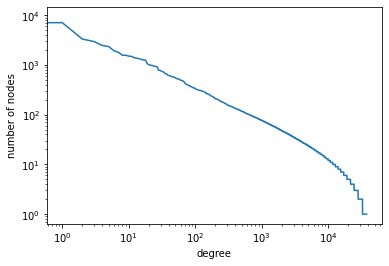
\includegraphics[scale=0.50]{charts/degree_dist_plot.png}
        \end{center}
    Plotting the histogram of degree distribution the following can be found:
    The chart clearly expose the difference in the degree distribution, mostly of the nodes are unknown but very few nodes are very popular, perhaps indicating that some power law can be present in the distribution of this measure. \\
    Using the module powerlaw from python the following chart of the cumulative distribution function (ccdf) is obtained:
    \begin{center}
    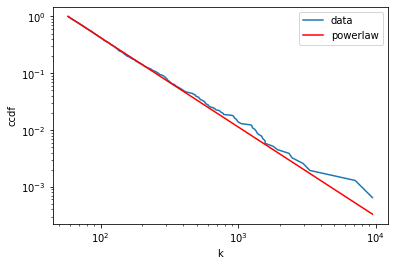
\includegraphics[scale=0.5]{charts/powerlaw.png}
    \end{center}
    In the chart the red line is the ccdf of a tipical powerlaw, meanwhile the blue line is the ccdf of the degree. Comparing the line is visible that the degree distribution is following a power law of type $f(k) \propto k^{-\alpha}$, the module also can estimate $\alpha$ that assumed the value 2.5733, meaning that the degree distribution is not only a power law but is also in the scale free regime because the exponent is in the interval [2,3].
    %% TODO include demonstration of this fact here

    \section*{Assortativity Measures}
    \subsection*{Clustering Coefficient}
    The analysis of Clustering Coefficient was computer using the networkx.clustering function that just follows the formula 
    $C(i)= \frac{\tau(i)}{\tau_{\max}} = \frac{2\tau_i}{k_i(k_i-1)}$ , or in latter words the ratio between traingles present around the node i $\tau_i$ and the maximum possible value of traingles that can be around i $\tau_{\max}$ . The distribution of this measure is the following: 
    \begin{center}
        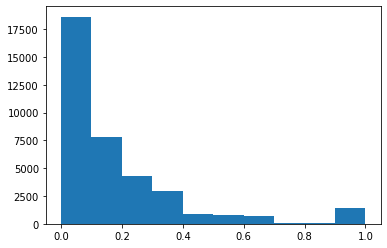
\includegraphics[scale=0.5]{charts/cc_distr.png}
    \end{center}
    It seems that over half of the nodes has no triangles, while there are very very few that have the maximum value possible. So it's a network with few spot that are connected to a great quantity of leafs , resembling an hub and spoke shape. While it's unusual in a social network this behaviour can be caused by the architecture of Github itself, usually for big projects (like big tech companies open source releases) a user is created and contains the repositiories not only of the interested project but also plugins and third party, so when for example a Unreal Engine developer wants to download the update directly from the repository and compile it itself he follow the user proprietary of such project, in this way he will be notified if a new update has been released (this happens for example also for Tensorflow, a Tensorflow user exists and also it is the owner of the project). But in this network the edges are mutual relationships, so the hypothesis can be that leafs are employed people working on a repository, the hub are companies or user that hold that project that follow the direct contributors of the project itself, maybe in order to track the progress on theyr forks or private branch.

    \subsection*{Degree Correlation}
    In order to understand better assortativity, let's plot the degree correlation function using the definition of $k_{nn}(i)= \frac{1}{k_i}\sum_j(a_{ij}k_j)$ as the average degree of the neighbours of node i and $k_{nn}(k) = <k_{nn}(i)>_{i:k_i=k}$ as the average degree of neighbours of node i that have degree k.
    \begin{center}
        \includegraphics*[scale=0.5]{charts/assort_plot.png}
    \end{center}
    From the chart is evident that this network is a metabolic disassortative network, confirming the previous hypothesis on the hub and spoke shape. 
    %%TODO maybe a more prolific discussion is required

    \subsection*{Homophily} 
    Let's analyze the homophily between the 2 groups categorized in the network: machine network developers and web developers. The total number of ML developers are: 9739 meanwhile the number of web developers are: 27961, the number of cross edges is $8,9*10^4$, a simple formula to show if there is homophily or not is $N_{ce} < 2pq$ where N\_ce is the number of cross edges, p are ML developers and q are web developers. The number of cross edges is significantly less than 2pq= $ 2,7*10^8$ showing that homophily is in action.
    
    \section*{Distances}  
    \subsection*{Distances Distribution}
    Using BFS let's calculate the distances starting from node 0:
    \begin{center}
        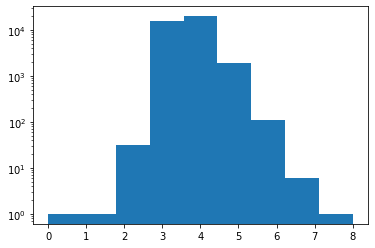
\includegraphics[scale=0.5]{charts/distances.png}
    \end{center}
    The chart show that most of the nodes have distance 4 and other significant measures are in the round of that value.

    %%TODO maybe the average path length goes there

    \subsection*{Centralities}
    Targeting the importance of nodes the first thing is calculate the closeness: $g_i = \frac{1}{\sum_{j!=i}l_{[ij]}}$
    \begin{center}
        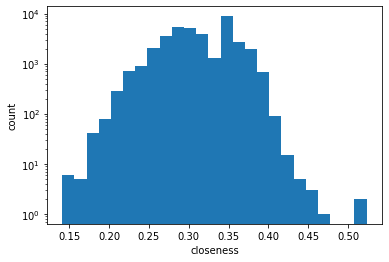
\includegraphics[scale=0.5]{charts/closeness_dist.png}
    \end{center}
    The distribution assumed by values resembled a normal distribution, with in center the mean of values:
    \begin{itemize}
        \item Mean: 0.3136
        \item Max: 0.5230
        \item Min: 0.1413
        \item Variance: 0.0016
    \end{itemize}
    Also the explicit result of those statistical values is confirming the hypothesis that the distribution is a normal like one, so the bigger part of nodes are equally closer to each other. Let's explore now the betwenness , using the estimated betwenness algorithm of the networkit package the following distribution is plotted:
    \begin{center}
        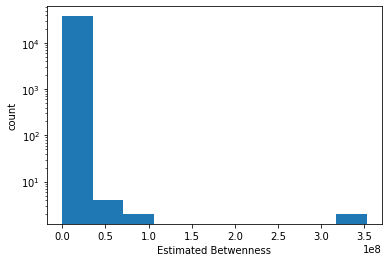
\includegraphics[scale=0.5]{charts/ebtw_dist.png}
    \end{center}
    It seems that what had been told for the closeness can be said for the betwenness, in fact most of the nodes seems to have 0 flow, meaning that no shortest path cross them at all, meanwhile there are very few nodes with the maximum value, this could mean that remove them will crash the network functionality. Let's compare the result of estimated betwenness with the exact one :
    \begin{center}
        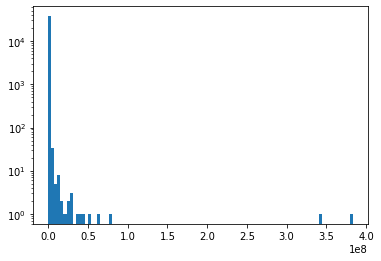
\includegraphics{charts/btw_dist.png}
    \end{center}
    the distributions are similiar, sypthom that the estimated betwenness perform quite well in estimating the value of the exact betwenness despite the lack of theoretical proof that ebtw works. Let's exploit the context to explain the causes of the behaviour of those two measures. Nodes are (for the bigger part) equally closer one to each other , this is compatible with the context, most of the nodes are employers working on common repositiories, so expect for the holders of those repositiories most of the nodes are leafs. Same could be say for the betwenness, most of the nodes aren't important at all, except for hubs of big projects, for example the maximum value of betwenness is reached in this network by node 31890 (dalinhuang99) former holder of paypaw project, a platform for exchange bitcoins (now not present anymore).

    \section*{Communities} 

    

\end{document}